% !TeX root = ./Dyplom.tex

\chapter{Projekt aplikacji}
\section{Strona internetowa}
	Do stworzenia strony zdecydowano się użyć frameworku Angular 8.
	Serwowana będzie ze środowiska uruchomieniowego Node.js.
	Projekt zbudowany jest z osobnych modułów dla każdej funkcjonalności.
	Widoki składane są z komponentów --- są to elementy zawierające szablon HTML, style CSS oraz logikę i dane w klasie napisanej w języku typescript.
	Dodatkowo komponenty mogą korzystać z serwisów. Serwisy to specjalne klasy, które są wstrzykiwane jako zależności (ang \emph{Dependency injection}).
	Zawierają się w nich dane oraz logika dzielone między wieloma komponentami.
	Nawigacja pomiędzy poszczególnymi widokami odbywa się przy pomocy dedykowanego routera, który przechwytuje nawigację przeglądarki.
	Dzięki temu nawet nawigacja do tyłu nie powoduje przeładowania całej strony tylko poszczególnych zmienionych elementów.

	Do budowy widoków użyta zostanie biblioteka Angular Material,
	która zawiera często wykorzystywane elementy zbudowane zgodnie z oficjalną specyfikacją \emph{Material design}.

	Taka modularna architektura pozwala na wielokrotne używanie tych samych komponentów oraz na zachowanie czytelnej struktury kodu.

\section{Serwis API}
	Projekt podzielony zostanie na trzy warstwy:
	\begin{description}
		\item[Api] warstwa obsługująca zapytania GraphQL
		\item[Core] warstwa domenowa definiująca modele encji, serwisy oraz interfejsy, z których korzysta warstwa Api
		\item[Infrastructure] warstwa implementująca interfejsy oraz obsługująca dostęp do bazy danych
	\end{description}

	Podział ten znany jest jako ,,czysta architektura'' (ang.\ \emph{Clean architecture}).
	Schemat ten przedstawiony został na rysunku~\ref{fig:cleanArch},
	gdzie linie ciągłe oznaczają zależności na etapie budowania, natomiast linia przerywana oznacza zależność po uruchomieniu.
	Taki układ umożliwia umieszczenie logiki biznesowej oraz modelu aplikacji w centrum (Core).
	W ten sposób infrastruktura oraz szczegóły implementacji są zależne od Core, a nie na odwrót --- odwrócenie zależności.
	Warstwa API pracuje na interfejsach zdefiniowanych w Core i nie zna ich implementacji w Infrastructure.
	Implementacje te są podłączane dopiero po uruchomieniu poprzez wstrzykiwanie zależności.
	Istotną zaletą takiej architektury jest również możliwość testowania każdej funkcjonalności z osobna.

	\begin{figure}[ht]
		\centering
			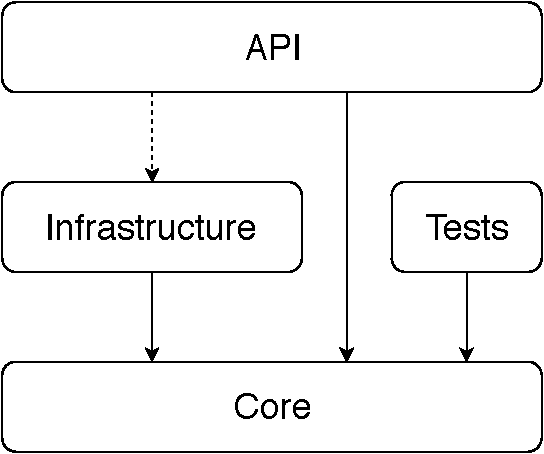
\includegraphics[width=0.3\linewidth]{rys03/CleanArch.pdf}
		 \caption{Schemat czystej architektury użyta w projekcie}
		 \label{fig:cleanArch}
	\end{figure}

	Na platformie \@.Net Core dostępne są dwie aktywnie rozwijane biblioteki implementujące GraphQL\@: \emph{GraphQL \@.NET} oraz \emph{Hot Chocolate}.
	Mimo znacznie mniejszej popularności wybrana została biblioteka \emph{Hot Chocolate},
	ponieważ prezentuje wiele możliwości automatyzacji generowania schematu GraphQL\@ oraz analizowania zapytań.

	Z racji tego, że GraphQL jest protokołem służącym do przesyłania danych, jest on zaimplementowany w najwyższej warstwie serwisu -- Api.
	W związku z tym nie zawęża sposobu implementacji zapisu danych w warstwie infrastruktury,
	a więc nic nie stoi na przeszkodzie, aby użyć relacyjnej bazy SQL.
	Takie rozwiązanie umożliwia wykorzystanie zalet relacyjnych baz - integralność i niezależność danych,
	jednocześnie oferując grafowy odczyt danych poprzez GraphQL.

\section{Baza danych}
	Baza danych stworzona zostanie w systemie zarządzania relacyjną bazą danych PostgreSQL.
	Jest to open source'owe oprogramowanie, obecnie jeden z najlepiej rozwiniętych RDBMS-ów.

	Baza z kontami użytkowników (rys.~\ref{fig:erdAuth}) zostanie wygenerowana za pomocą platformy Identity.
	Tabele te przechowują podstawowe dane kont użytkowników takie jak login, hasz hasła czy email.
	Zawierają się tu również role oraz ich upoważnienia (opisane szerzej w rozdziale !!!!WSTAWIĆ TU ref DO ROZDZIAŁU !!!!!!!!!!!!!!!!!!!!!!!!!!!!!!!!).
	Oprócz danych użytkowników zapisywane są również dane związane z migracjami bazy zarządzane przez \emph{Entity Framework}
	oraz dwie pomocnicze tabele biblioteki \emph{IdentityServer4} (\emph{DeviceCodes} i \emph{PersistedGrants}).

	\begin{figure}[ht]
		\centering
			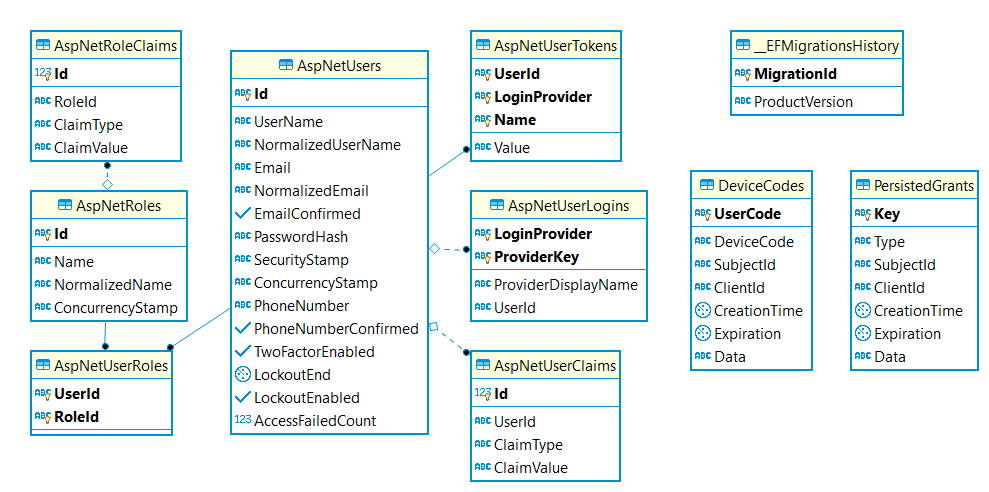
\includegraphics[width=\linewidth]{rys03/erdAuth.png}
		 \caption{Schemat ERD bazy z kontami użytkowników}
		 \label{fig:erdAuth}
	\end{figure}
	
	Rysunek~\ref{fig:erdRe} przedstawia bazę przechowującą główne dane aplikacji.
	Przechowywana jest minimalna ilość danych wymagana do zaimplementowania wersji konceptualnej aplikacji.
	Jeśli aplikacja miałaby zostać wdrożona, z konieczne byłoby dodanie większej ilości danych.
	Tabele połączone są relacjami umożliwiającymi grafową reprezentację.
	Baza ta również została wygenerowana metodą code first za pomocą \emph{Entity Framework}.

	\begin{figure}[ht]
		\centering
			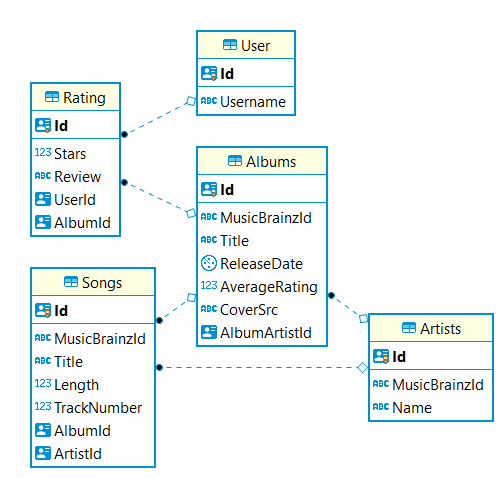
\includegraphics[width=0.5\linewidth]{rys03/erdRe.png}
		 \caption{Schemat ERD bazy z głównymi danymi}
		 \label{fig:erdRe}
	\end{figure}

\section{Uwierzytelnianie i autoryzacja}
	Jako protokół uwierzytelniania wybrano OpenID Connect.
	Standard ten rozszerza OAuth2 (służący do autoryzacji) o warstwę identyfikacji użytkowników.
	Jest obecnie jednym z najbezpieczniejszych standardów uwierzytelniania.
	Zaimplementowany zostanie przy pomocy biblioteki \emph{IdentityServer4} na platformie \emph{ASP.Net Core 3.0}.
	Użytkownik po zalogowaniu otrzyma token JWT, który będzie zawierał cyfrową sygnaturę.
	Dzięki temu jakakolwiek ingerencja w jego strukturę sprawi, iż jego walidacja zakończy się niepowodzeniem.

	Dla zapewnienia najwyższego standardu bezpieczeństwa zaimplementowany zostanie proces logowania z wykorzystaniem kodu PKCE (ang.\ \emph{Proof Key for Code Exchange}),
	opisany w dokumencie RFC~7636~\cite{PKCE}.
	Stanowi on udoskonalenie przepływu wykorzystującego kod autoryzacji (ang.\ \emph{Authorization Code Flow}).
	Zabezpiecza przed próbami przechwycenia kodu autoryzacji przez złośliwą aplikację,
	która mogła by za pomocą tego kodu uzyskać token dostępowy (ang.\ \emph{Access Token}).
	
	Proces uzyskania tokenu dostępowego, przedstawiony na schemacie~\ref{fig:pkce}, jest następujący:
	\begin{enumerate}[label=\Alph*.]
		\item Klient tworzy losowy klucz \verb|code_verifier| i przekształca go za pomocą metody transformacji \verb|t_m|.
			Następnie przesyła przekształcony klucz wraz z metodą transformacji w żądaniu autoryzacji OAuth 2.0.
		\item Jeśli użytkownik zalogował się poprawnymi danymi, serwer zapisuje parametry weryfikacji i zwraca kod autoryzacji.
		\item Aby uzyskać token dostępowy, klient przesyła kod autoryzacji wraz z oryginalną wartością \verb|code_verifier| wygenerowaną w punkcie (A).
		\item Serwer autoryzacji przekształca \verb|code_verifier| za pomocą metody \verb|t_m|
			i porównuje z wartością \verb|t(code_verifier)| otrzymaną w punkcie (B).
			Jeśli są równe, serwer zwraca token dostępowy.
	\end{enumerate}

	W ten sposób nawet jeśli kod autoryzacji w punkcie (B) zostanie przechwycony,
	nie będzie mógł zostać wykorzystany bez znajomości klucza \verb|code_verifier|.

	\begin{figure}[ht]
		\centering
			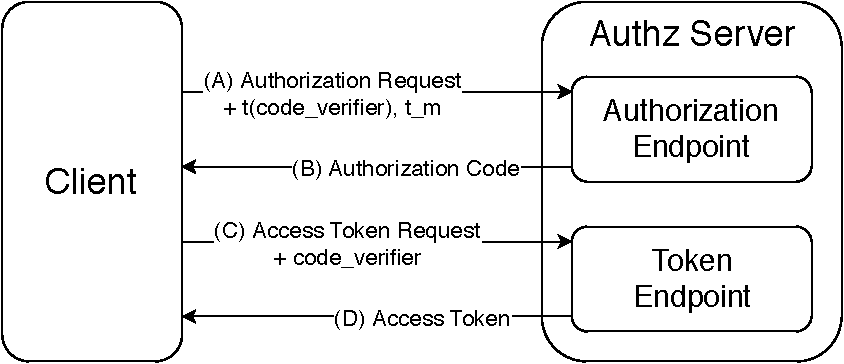
\includegraphics[width=0.7\linewidth]{rys03/pkce.pdf}
		 \caption{Schemat procesu logowania z użyciem PKCE}
		 \label{fig:pkce}
	\end{figure}
